\let\negmedspace\undefined
\let\negthickspace\undefined
\documentclass[journal]{IEEEtran}
\usepackage[a5paper, margin=10mm, onecolumn]{geometry}
%\usepackage{lmodern} % Ensure lmodern is loaded for pdflatex
\usepackage{tfrupee} % Include tfrupee package

\setlength{\headheight}{1cm} % Set the height of the header box
\setlength{\headsep}{0mm}     % Set the distance between the header box and the top of the text

\usepackage{gvv-book}
\usepackage{gvv}
\usepackage{cite}
\usepackage{amsmath,amssymb,amsfonts,amsthm}
\usepackage{algorithmic}
\usepackage{graphicx}
\usepackage{textcomp}
\usepackage{xcolor}
\usepackage{txfonts}
\usepackage{listings}
\usepackage{enumitem}
\usepackage{mathtools}
\usepackage{gensymb}
\usepackage{comment}
\usepackage[breaklinks=true]{hyperref}
\usepackage{tkz-euclide} 
\usepackage{tikz}
\usepackage{listings}
\usetikzlibrary{patterns}
% \usepackage{gvv}                                        
\def\inputGnumericTable{}                                 
\usepackage[latin1]{inputenc}                                
\usepackage{color}                                            
\usepackage{array}                                            
\usepackage{longtable}                                       
\usepackage{calc}                                             
\usepackage{multirow}                                         
\usepackage{hhline}                                           
\usepackage{ifthen}                                           
\usepackage{lscape}
\begin{document}
\bibliographystyle{IEEEtran}
\vspace{3cm}

\title{GATE\\CE - 2017}
\author{EE24BTECH11061 - Rohith Sai}
\maketitle

\renewcommand{\thefigure}{\theenumi}
\renewcommand{\thetable}{\theenumi}

\section*{Single Correct 2 Marks each}
\begin{enumerate}
\item The solution of the equation $\frac{dQ}{dt} + Q = 1$ with $Q = 0$ at $t=0$ is
\begin{multicols}{2}
    \begin{enumerate}
        \item $Q\brak{t} = e^{-t} - 1$
        \item $Q\brak{t} = 1 + e^{-t}$
        \item $Q\brak{t} = 1 - e^{t}$
        \item $Q\brak{t} = 1 - e^{-t}$
    \end{enumerate}
\end{multicols}

\item Consider the matrix $\myvec{5 & -1\\4 & 1}$. Which of the following statements is TRUE for the eigenvalues and eigenvectors of this matrix?
\begin{multicols}{2}
    \begin{enumerate}
        \item Eigenvalue 3 has a multiplicity of 2, and only one independent eigenvector exists.
        \item Eigenvalue 3 has a multiplicity of 2, and two independent eigenvectors exist.
        \item Eigenvalue 3 has a multiplicity of 2, and no independent eigenvector exists.
        \item Eigenvalues are 3 and -3, and two independent eigenvectors exist.
    \end{enumerate}
\end{multicols}
    
\item A planar truss tower structure is shown in the figure\\
\begin{center}
\begin{tikzpicture}
    %own code
    \draw[thick, double, line width = 0.8pt] (-0.5,0) -- (0.5,0);
    \draw[thick, double, line width = 0.8pt] (-0.5,0) -- (-1,-1.5);
    \draw[thick, double, line width = 0.8pt] (0.5,0) -- (1,-1.5);
    \draw[thick, double, line width = 0.8pt] (-0.5,0) -- (1,-1.5);
    \draw[thick, double, line width = 0.8pt] (0.5,0) -- (-1,-1.5);
    \draw[thick, double, line width = 0.8pt] (-1,-1.5) -- (1,-1.5);
    \draw[thick, double, line width = 0.8pt] (-1,-1.5) -- (-1.5,-3);
    \draw[thick, double, line width = 0.8pt] (-1,-1.5) -- (1.5,-3);
    \draw[thick, double, line width = 0.8pt] (1,-1.5) -- (-1.5,-3);
    \draw[thick, double, line width = 0.8pt] (1,-1.5) -- (1.5,-3);
    \draw[thick, double, line width = 0.8pt] (-1.5,-3) -- (1.5, -3);

    \draw[thick] (-1.5,-3) -- (-1.8,-3.5) -- (-1.2,-3.5) -- cycle;
    \draw[thick] (1.5,-3) -- (1.8,-3.5) -- (1.2,-3.5) -- cycle;

\end{tikzpicture}
\end{center}
Consider the following statements about the external and internal determinacies of the truss.\\
(P) Externally Determinate\\
(Q) External Static Indeterminacy = 1\\
(R) External Static Indeterminacy = 2\\
(S) Internally Determinate\\
(T) Internal Static Indeterminacy = 1\\
(U) Internal Static Indeterminacy = 2\\
Which one of the following options is correct?
\begin{multicols}{2}
    \begin{enumerate}
        \item P-False; Q-True; R-False; S-False; T-False; U-True
        \item P-False; Q-True; R-False; S-False; T-True; U-False
        \item P-False; Q-False; R-True; S-False; T-False; U-True
        \item P-True; Q-True; R-False; S-True; T-False; U-True
    \end{enumerate}
\end{multicols}

\item Group I contains three broad classes of irrigation supply canal outlets. Group II presents hydraulic performance attributes.
\begin{center}
    \begin{tabular}{|c|c|c|} 
        \hline
            \textbf{Variable} & \textbf{Description} & \textbf{Value} \\ 
        \hline
            $\vec{a}$    & Length of $BC$ & $6cm$ \\ 
        \hline
            $\vec{b}$    & Length of $AC$ & $?$\\ 
        \hline
            $\vec{c}$    & Length of $AB$ & $5cm$\\
        \hline
            $\angle{ABC}$& Angle $B$      & $60\degree$\\
        \hline
    \end{tabular}
\end{center}
\begin{multicols}{2}
    \begin{enumerate}
        \item P-1; Q-2; R-3
        \item P-3; Q-1; R-2
        \item P-2; Q-3; R-1
        \item P-1; Q-3; R-2
    \end{enumerate}
\end{multicols}

\item A 1 m wide rectangular channel has a bed slope of 0.0016 and the Manning's roughness coefficient is 0.04. Uniform flow takes place in the channel at a flow depth if 0.5 m. At a particular section, gradually varied flow (GVF) is observed and the flow depth is measured as 0.6 m. The GVF profile at that section is classified as
\begin{multicols}{2}
    \begin{enumerate}
        \item $S_1$
        \item $S_2$
        \item $M_1$
        \item $M_2$
    \end{enumerate}
\end{multicols}

\item The following observations are made while testing aggregate for its suitability in pavement construction:\\
i. Mass of oven-dry aggregate in air = 1000 g\\
ii. Mass of saturated surface-dry aggregate in air = 1025 g\\
iii. Mass of saturated surface-dry aggregate under water = 625 g\\
Based on the above observations, the correct statement is
\begin{multicols}{2}
    \begin{enumerate}
        \item bulk specific gravity of aggregate = 2.5 and water absorption = 2.5\%
        \item bulk specific gravity of aggregate = 2.5 and water absorption = 2.4\%
        \item apparent specific gravity of aggregate = 2.5 and water absorption = 2.5\%
        \item apparent specific gravity of aggregate = 2.5 and water absorption = 2.4\%
    \end{enumerate}
\end{multicols}

\item The queue length (in number of vehicles) versus time (in seconds) plot for an approach to a signalized intersection with the cycle length of 96 seconds is shown in the figure (not drawn to scale).
\begin{figure}[h!]
    \centering
    \includegraphics[width=0.5\linewidth]{figs/figure.png}
    \label{fig:enter-label}
\end{figure}\\
At time $t=0$, the light has just turned red. The effective green time is 36 seconds, during which vehicles discharge at the saturation flow rate, $s$ (in vph). Vehicles arrive at a uniform rate, $v$ (in vph), throughout the cycle. Which one of the following statements is TRUE?
\begin{multicols}{2}
    \begin{enumerate}
        \item $v = 600$ vph, and for this cycle, the average stopped delay per vehicle = 30 seconds 
        \item $s = 1800$ vph, and for this cycle, the average stopped delay per vehicle = 28.125 seconds 
        \item $v = 600$ vph, and for this cycle, the average stopped delay per vehicle = 45 seconds 
        \item $s = 1200$ vph, and for this cycle, the average stopped delay per vehicle = 28.125 seconds
    \end{enumerate}
\end{multicols}

\item The radius of a horizontal circular curve on a highway is 120 m. The design speed is 60 km/hour, and the design coefficient of lateral friction between the tyre and the road surface is 0.15. The estimated value of superelevation required (if full lateral friction is assumed to develop), and the value of coefficient of friction needed (if no superelevation is provided) will, respectively, be
\begin{multicols}{2}
    \begin{enumerate}
        \item $\frac{1}{11.6}$ and 0.10
        \item $\frac{1}{10.5}$ and 0.37
        \item $\frac{1}{11.6}$ and 0.24
        \item $\frac{1}{12.9}$ and 0.24
    \end{enumerate}
\end{multicols}

\item The observed bearings of a traverse are given below:
\begin{table}[h!]
    \centering
    \begin{tabular}{|c|c|@{\hskip 10pt}|c|c|}
        \hline
        \textbf{Line} & \textbf{Bearing} & \textbf{Line} & \textbf{Bearing} \\
        \hline
        PQ & 46$^\circ$15' & QP & 226$^\circ$15' \\
        \hline
        QR & 108$^\circ$15' & RQ & 286$^\circ$15' \\
        \hline
        RS & 201$^\circ$30' & SR & 20$^\circ$30' \\
        \hline
        ST & 321$^\circ$45' & TS & 141$^\circ$45' \\
        \hline
    \end{tabular}
\end{table}


The station(s) most likely to be affected by the local attraction is/are
\begin{multicols}{2}
    \begin{enumerate}
        \item only R
        \item only S
        \item R and S
        \item P and Q
    \end{enumerate}
\end{multicols}

\item The laboratory tests on a soil sample yields the following results: natural moisture content = 18\%, liquid limit = 60\%, plastic limit = 25\%, percentage of clay sized fraction = 25\%.\\
The liquidity index and activity (as per the expression proposed by Skempton) of the soil, respectively, are
\begin{multicols}{2}
    \begin{enumerate}
        \item -0.2 and 1.4
        \item 0.2 and 1.4
        \item -1.2 and 0.714
        \item 1.2 and 0.714
    \end{enumerate}
\end{multicols}

\item Consider the equation $\frac{du}{dt} = 3t^2 + 1$ with $u=0$ at $t=0$. This is numerically solved by using the forward Euler method with a step size, $\delta t = 2$. The absolute error in the solution at the end of the first time step is \rule{1cm}{0.15mm} .

\item A pre-tensioned rectangular concrete beam 150 mm wide and 300 mm depth is prestressed with three straight tendons, each having a cross-sectional are of 50 mm${^2}$, to an initial stress of 1200 N/mm${^2}$. The tendons are located at 100 mm from the soffit of the beam. If the modular ratio is 6, the loss of prestressing force (in kN, up to one decimal place) due to the elastic deformation of concrete only is \rule{1cm}{0.15mm}

\item Consider the stepped bar made with a linear elastic material and subjected to an axial load of 1 kN, as shown in the figure.
\begin{tikzpicture}[scale=0.7]
    \draw[thick] (-2, 0) -- (2, 0);
    \draw[thick] (-2, 0) -- (-2, 0.2) -- (2, 0.2) -- (2, 0);
    \foreach \x in {-1.9,-1.7,...,1.9}
        \draw[thick] (\x, 0.2) -- (\x + 0.1, 0);

    % Draw block 1
    \draw[thick] (-1.2, 0) -- (-1.2, -3);
    \draw[thick] (1.2, 0) -- (1.2, -3);
    \draw[thick] (-1.2, -3) -- (1.2, -3);

    % Draw block 2
    \draw[thick] (-0.8, -3) -- (-0.8, -7);
    \draw[thick] (0.8, -3) -- (0.8, -7);
    \draw[thick] (-0.8, -7) -- (0.8, -7);

    % Dimensions and labels
    % Labels for block 1
    \node at (0, -1.5) {1};
    \node at (3.5, -1) {$A_1 = 100\ \mathrm{mm^2}$};
    \node at (3.5, -2) {$E_1 = 2 \times 10^5\ \mathrm{MPa}$};

    % Labels for block 2
    \node at (0, -5) {2};
    \node at (3.5, -4) {$A_2 = 60\ \mathrm{mm^2}$};
    \node at (3.5, -5) {$E_2 = 3 \times 10^5\ \mathrm{MPa}$};

    % Dimensions on the left side
    \draw[<->] (-2, 0) -- (-2, -3);
    \node[left] at (-2.5, -1.5) {$L_1 = 400\ \mathrm{mm}$};

    \draw[<->] (-2, -3) -- (-2, -7);
    \node[left] at (-2.5, -5) {$L_2 = 900\ \mathrm{mm}$};

    % Load arrow at the bottom
    \draw[thick, ->] (0, -7) -- (0, -9);
    \node[right] at (0, -8) {$P = 1\ \mathrm{kN}$};
\end{tikzpicture}\\
Segments 1 and 2 have cross-sectional area of 100 mm$^{2}$ and 60 mm$^2$, Young's modulus of $2 \times 10^5$ Mpa and $3 \times 10^5$ MPa, and length of 400 mm and 900 mm, respectively. The strain energy (in N-mm, up to one decimal place) in the bar due to the axial load is \rule{1cm}{0.15mm}
\end{enumerate}
\end{document}